\documentclass[a4paper, 11pt]{scrartcl}
\usepackage[utf8]{inputenc}
\usepackage[english]{babel}
\usepackage[T1]{fontenc}
\usepackage{amsmath}
\usepackage{graphicx}
\usepackage{url}
\usepackage{float}
\usepackage{fancyhdr}
\bibliographystyle{plainnat}
\newcommand{\uproman}[1]{\uppercase\expandafter{\romannumeral#1}}

\title {Delevopment of a 2D Galvo laser engraver}
\author {Niklas H}
\date {\today}

\begin{document}
\maketitle
\tableofcontents
\newpage

\section{Introduction}
In this documentation, the construction of a Galvo-style high-speed laser engraver will be discussed. The goal is to upgrade the existing device to a user friendly laser engraver with high engraving speed.

\section{Theory}
In this section, relevant theory will be discussed. The development of the scanner will be based on these details. \\
\subsection{Laser diodes} 

\subsection{Stepper motors}

\subsection{Optics of the scanner} 


\section{Implementation}
In this section, construction details of the galvo scanner will be explained.
\subsection{Mechanics and Optics}
\begin{figure}[H]
\begin{center}
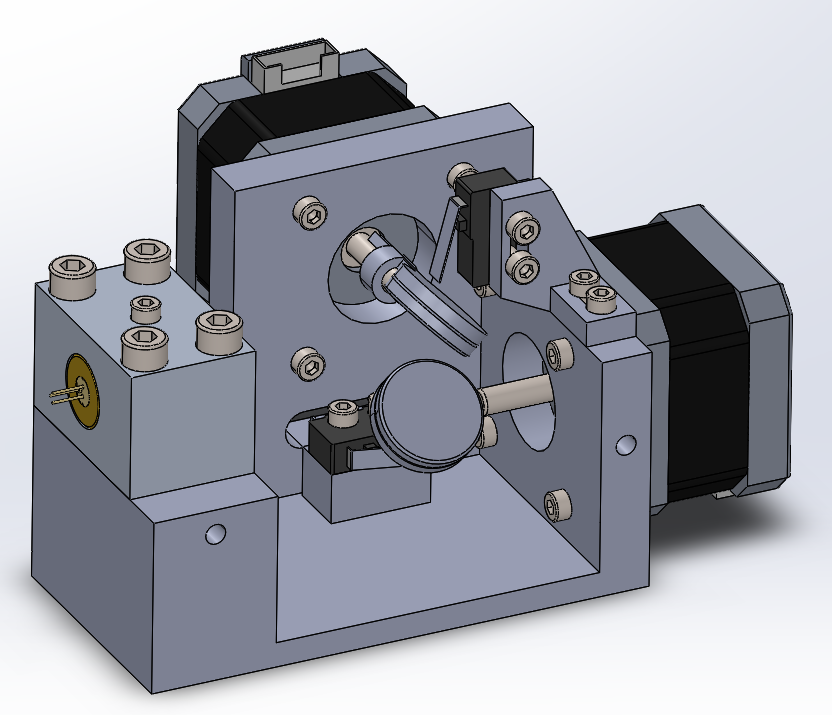
\includegraphics[width=15cm]{img/mechanics.png}
\caption{CAD-Rendering of the mechanical system}
\label{mechanics}
\end{center}
\end{figure}

\addcontentsline{toc}{section}{References}
\bibliography{literature}
\end{document}